%%%%%%%%%%%%%%%%%%%%%%%%%%%%%%%%%%%%%%%%%%%%%%%%%%%%
\chapter{Konzept}
\label{sec:Konzept}
%%%%%%%%%%%%%%%%%%%%%%%%%%%%%%%%%%%%%%%%%%%%%%%%%%%%
In der Analyse wurde herausgearbeitet, welche Aspekte bei der Entwicklung des Assistenzsystems für die modularen Anlagen berücksichtigt werden müssen. Die vielschichtigen Faktoren werden nun ins Konzept mit einbezogen. Dazu wird zunächst mit dem konzeptionellen Design herausgearbeitet, welche Funktionen konkret umgesetzt werden müssen und wie Nutzer und Assistenz miteinander interagieren. Darauf aufbauend erfolgt der Entwurf eines physikalischen Designs. In diesem wird ein Vorschlag geliefert, wie ein System zur Problemlösung aussehen kann.

\section{Konzeptuelles Design}
\todo{Einleitung?}
\begin{figure}[htbp]
\centering
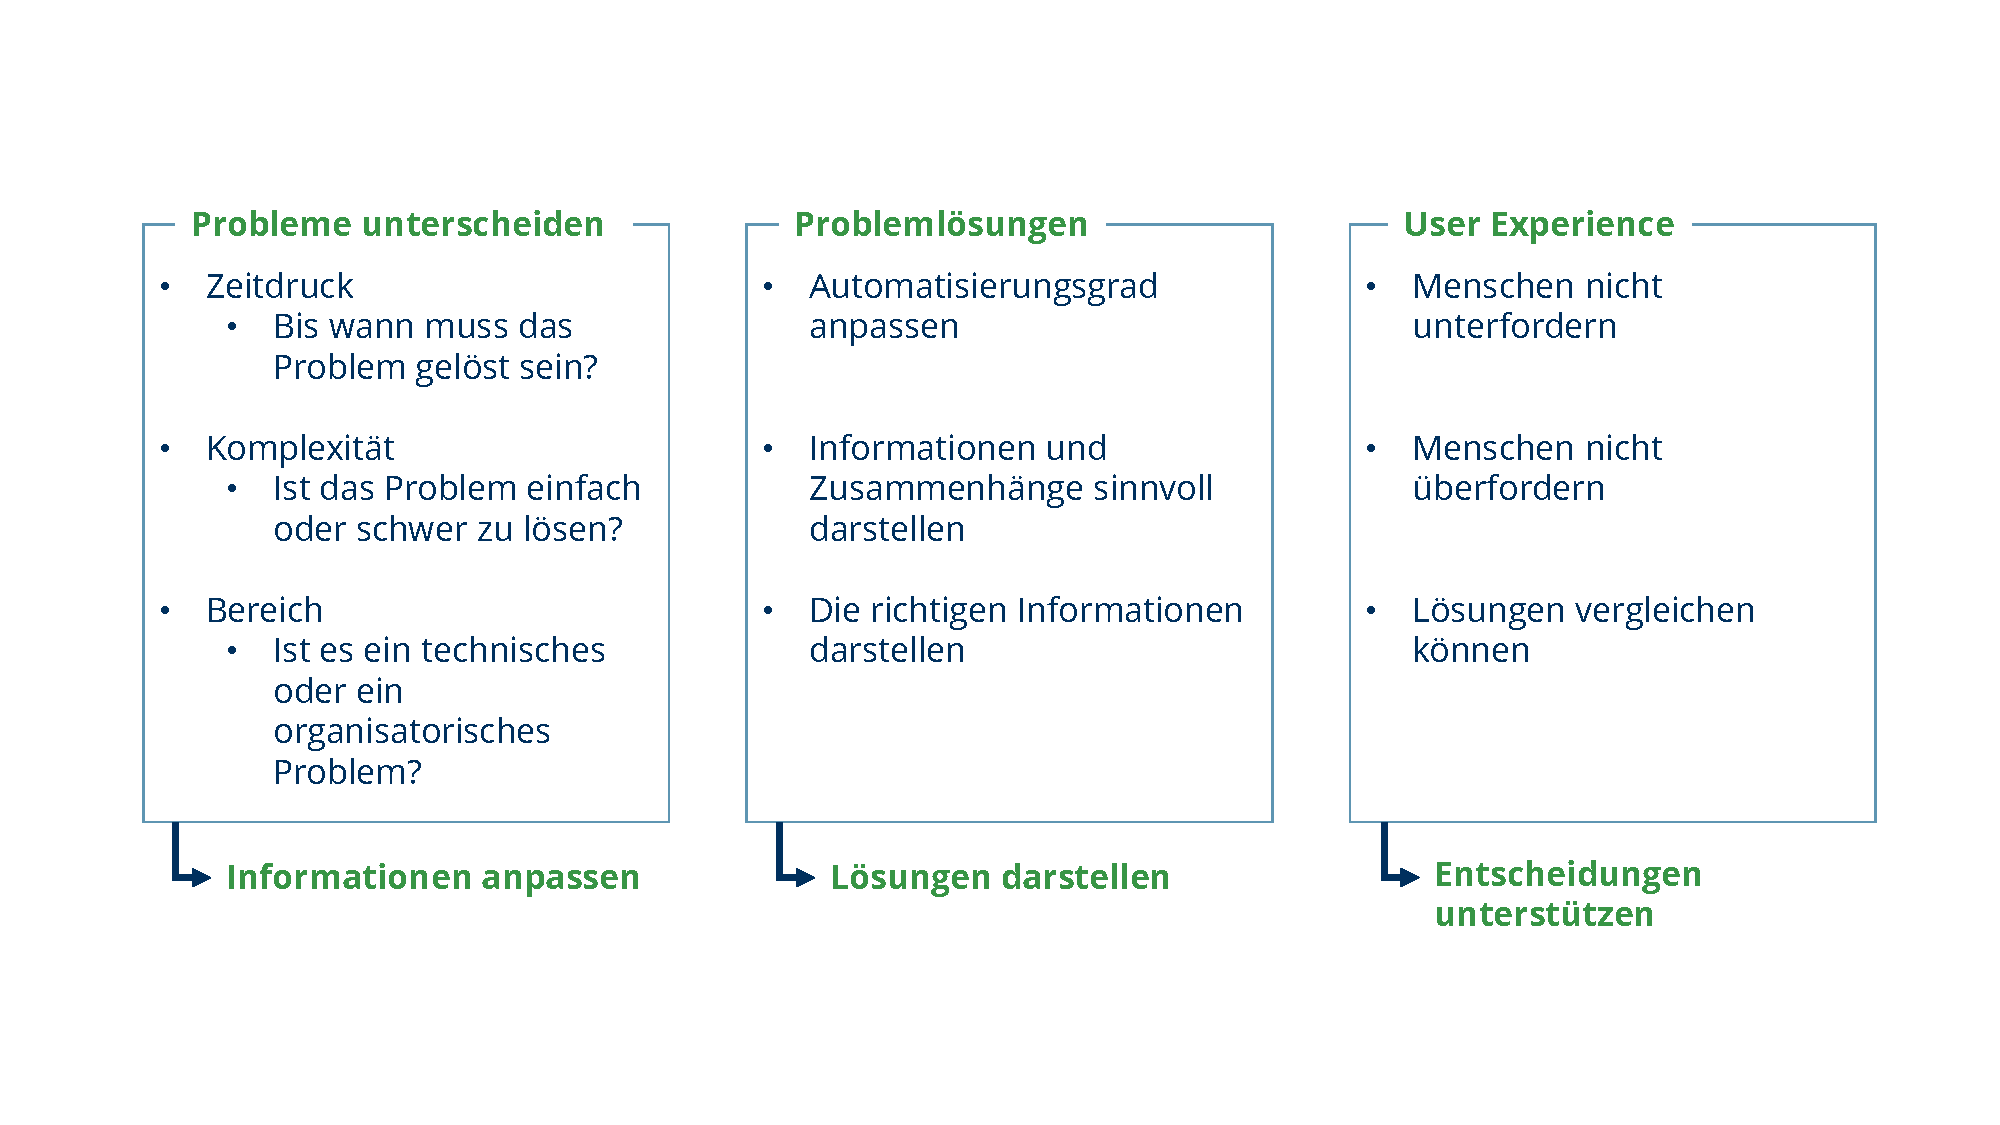
\includegraphics[scale=0.45]{DA_files/Bilder/Konzept/Nutzer-unterstuetzen.pdf}
\caption{Aspekte des Assistenzsystems}
\label{pic:Nutzer-Unterstuetzen}
\end{figure}
\\ \\
In Abschnitt \ref{2:Unterscheidung-Probleme} ist bereits aufgeführt, dass sich \textbf{Probleme unterscheiden}. Die Informationen sollen sich entsprechend dem Zeitdruck, der Komplexität des Problems und dem umfassenden Bereich automatisch anpassen. Dadurch soll sowohl eine Unterforderung, als auch eine Überforderung des Menschen verhindert werden.

Die \textbf{Lösungen für das Problem} sollen sinnvoll dargestellt werden. Dabei wird der Autonomiegrad anhand des Zeitdrucks angepasst. Die Menge an dargestellten Informationen und deren Zusammenhänge orientieren sich an der Komplexität des Problems. Die Komplexität des Problems lässt sich aus der Menge an Zusammenhängen ableiten. Deshalb ist es umso wichtiger diese strukturiert und klar darzustellen. Abhängig vom Bereich des Problems sind die richtigen Informationen darzustellen.

Mit einer guten \textbf{User Experience} soll die Entscheidung des Menschen unterstützt werden. Dieser soll mittels geeignetem Autonomiegrad nicht unterfordert werden. Durch die angemessene Darstellung der Informationen ist eine Überforderung zu vermeiden. Die Darstellung der Informationen hängt auch mit der Vergleichbarkeit der Lösungen zusammen. Gibt es mehrere Lösungen, so muss der Nutzer Unterschiede gut erkennen können, um eine geeignete Entscheidung zu treffen.
\\ \\
Wie kann nun der Nutzer durch den Problemlöseprozess begleitet werden? In Abschnitt \ref{2:Phasen-Problemloesen} sind die Phasen des Problemlösens beschrieben. Angelehnt daran wird folgender Ablauf mit entsprechender Unterstützung durch das Assistenzsystem vorgesehen (siehe Bild \ref{pic:Konzeptidee} \todo{Bild anpassen}).
\begin{figure}[htbp]
\centering
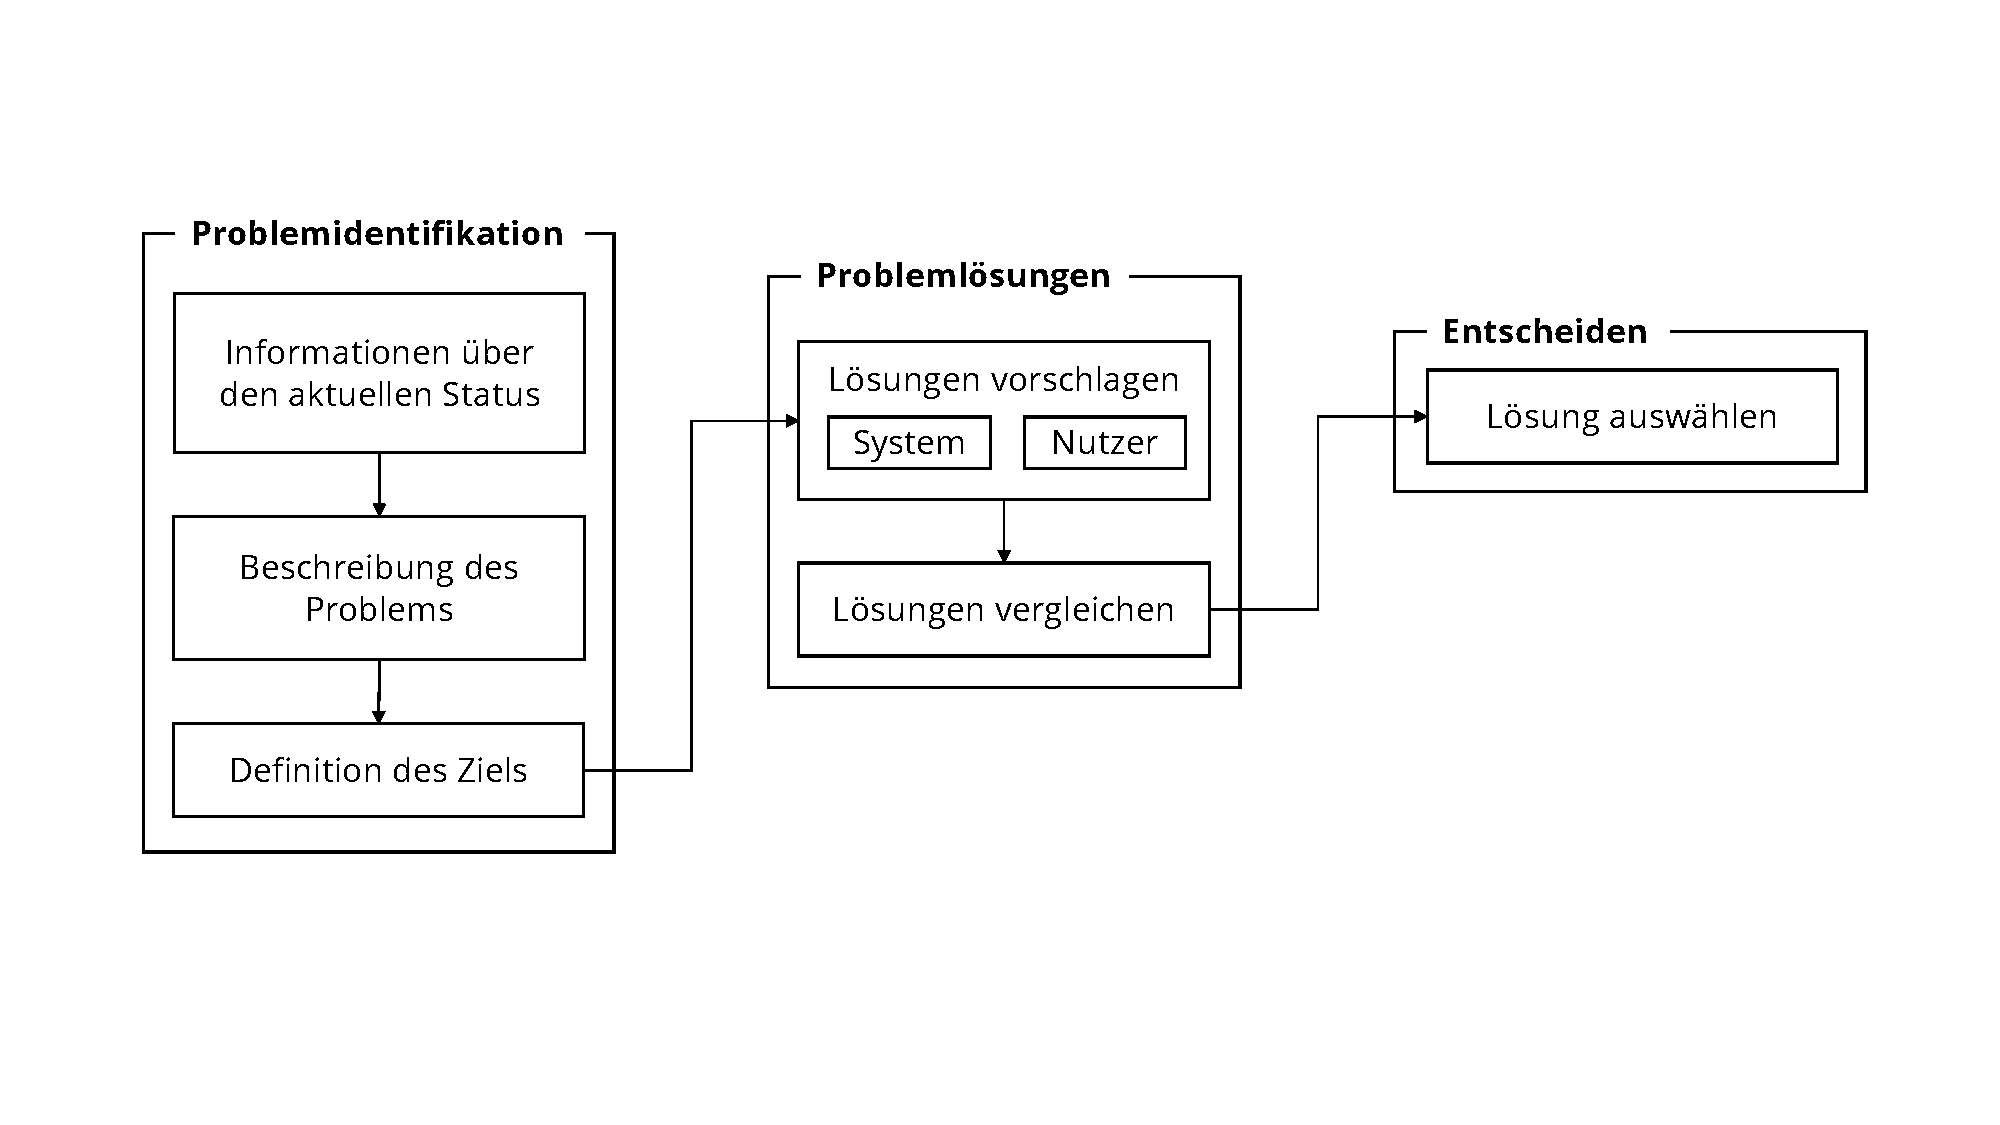
\includegraphics[scale=0.45]{DA_files/Bilder/Konzept/Konzeptidee.pdf}
\caption{Die Schritte des Problemlöseprozess}
\label{pic:Konzeptidee}
\end{figure}

Zunächst muss das Problem identifiziert werden. Dazu stehen dem Nutzer alle Informationen über den aktuellen Status der modularen Anlage zur Verfügung. Durch Meldungen, Warnungen und Alarme können Probleme vom System ausgelöst werden. Weiterführend ist es denkbar, dass auch der Nutzer ein Problem definiert. Ist das Problem identifiziert, so muss das Ziel definiert werden. Im Fall eines zu wartenden Moduls kann z.B. ein maximaler Produktionsausfall angegeben werden.

Ist das Problem identifiziert und das Ziel definiert, so müssen die möglichen Lösungen betrachtet werden. Lösungen können sowohl vom System, als auch vom Nutzer vorgeschlagen werden. Nach Bestimmung der Lösungen erfolgt ein Vergleich dieser.

Die Entscheidung für eine entsprechende Lösung wird mittels einer geeignete Darstellung durch das Assistenzsystem unterstützt. Wie dies aussehen kann ist in Abschnitt \ref{4:pD-Loesungen} dargestellt.

\subsection{Funktionen}
\todo{einleitenden Text schreiben}
Wie kann nun der oben beschriebene Problemlöseprozess unterstützt werden? Zunächst muss der Nutzer einen Überblick über den aktuellen Status erhalten. Taucht ein neues Problem auf so interagieren Nutzer und Assistent bis eine geeignete Lösung gefunden wird. Mehr dazu in Abschnitt xx.

\subsubsection*{Aktueller Status}
Der aktuelle Status kann über die PFE abgelesen werden. Diese gibt einen Überblick über die aktuelle Verschaltung der Module, das Rezept, die Key Performace Indicator (KPIs) und die Services. Auch eine Übersicht über das Anlagenequipment eines jeden Moduls ist vorhanden. Die notwendigen Meldungen, Warnungen und Alarme werden derzeit nicht angezeigt. Durch die Integration dieser kann der Nutzer bei der Problemidentifikation unterstützt werden. Tritt beispielsweise eine Meldung auf, hat der Nutzer die Möglichkeit dieses als Problem aufzunehmen und nach Lösungen zu suchen.

\subsubsection*{Neues Problem}
Welche Rahmenbedingungen sind für die Charakterisierung eines Problems relevant? In der Analyse (ref) wird sowohl auf die technischen, als auch die wirtschaftlichen Ziele verwiesen. Im Kontext eines produzierenden Unternehmens ist die Wirtschaftlichkeit eine wichtige ökonomische Zielgröße \cite{} (Bloech-Einführung in die Produktion). Dem Nutzer wird aus diesem Grund die Möglichkeit gegeben relevante Ziele hinzuzufügen und genauer zu spezifizieren. Welche dies genau sein können ist von dem Unternehmen und dem Problem abhängig.

Neben der Definition der Ziele, ist es dem Nutzer möglich eine Übersicht über den Problembereich zu erhalten. Dazu markiert das Assistenzsystem zunächst den Bereich in dem das Problem ausgelöst wurde und die zugehörigen Komponenten. Betrifft der Bereich ein bestimmtes Modul, dann werden die zugehörigen Services und der zugehörige Bereich im Rezept markiert. Betrifft der Bereich einen Service, sind die Parameterabhängigkeiten und das zugehörige Equipment relevant. Ausgehend von dem markierten Bereich und geleitet durch die Ziele können Lösungen gefunden werden.

\subsubsection*{Lösungen suchen}
Wie die konkrete Lösung für ein Problem aussieht ist nicht vorherbestimmt. Das Assistenzsystem kann anhand der definierten Ziele Vorschläge liefern. Diese können durch den Nutzer angepasst und bewertet werden. Hier ist der Mensch klar im Vorteil, da dieser Optionen abwägen kann. Des Weiteren hat der Nutzer die Möglichkeit selber nach Lösungen zu suchen. Ihm stehen dazu alle Informationen über die Anlage zur Verfügung. Das Assistenzsystem markiert die Veränderungen, die durch die Lösungen entstehen. Dadurch kann der Nutzer den Aufwand abschätzen und bewerten, ob die Lösung gut oder schlecht ist.

\subsubsection*{Lösungen vergleichen}
In vielen Fällen gibt es nicht nur eine richtige Lösung, sondern mehrere Lösungsmöglichkeiten, die gegeneinander abgewogen werden müssen. Dem Nutzer werden dazu die Unterschiede zwischen den Lösungen aufgezeigt. Diese können rein zahlenmäßig sein, wie entstehende Kosten oder die Länge des Stillstands. Es ist jedoch auch möglich, dass sich Lösungen strukturell unterscheiden, z.B. anhand der zur Verfügung gestellten Dienste. Durch einen Vergleich der Lösungen kann der Nutzer eine Entscheidung treffen und damit den Problemlöseprozess abschließen.

\subsection{Anpassungen an den Problembereich}
Da sich sowohl Probleme, als auch Lösungen von Fall zu Fall unterscheiden, müssen dementsprechend Anpassungen vorgenommen werden. In Abschnitt \ref{3:Anpassung-Aufgabe} ist bereits erwähnt, dass sich die Informationen an das Problem und die Ziele anpassen sollten. Im Zuge dessen sind vor allem die gegenseitigen Abhängigkeiten relevant, auf die im weiteren Verlauf näher eingegangen wird. Damit sich das Assistenzsystem anpassen kann muss identifiziert werden, wo das Problem entstanden ist. Es lassen sich folgende Fälle unterscheiden:
\begin{itemize}
\item \textbf{Modul:} Das gesamte Modul hat ein Problem verursacht.
\item \textbf{Service:} Ein Service hat eine Warnung oder Alarm ausgelöst.
\item \textbf{Rezept:} Das Rezept ist an einer bestimmten Stelle hängen geblieben und kann nicht weiter abgearbeitet werden.
\item \textbf{KPI:} Die KPI weisen Unregelmäßigkeiten auf oder erreichen vorher definierte Grenzwerte.
\end{itemize}

\subsubsection*{Modul}
Ein einzelnes Modul ist sehr eigenständig, da es grundsätzlich auch alleine betrieben werden kann. In der Navigation der PFE ist ersichtlich mit welchen anderen Modulen es verbunden ist. Um eine Problemlösung auf Modulebene zu unterstützen ist es notwendig die zugehörigen Services und den Bereich im Rezept zu markieren. Dadurch kann der Nutzer die Abhängigkeiten erkennen. 

\subsubsection*{Services}
Die Services weisen eine Vielzahl an Abhängigkeiten auf. So kann ein Service direkt mit anderen Services gekoppelt sein (vgl. Abschnitt \ref{2:Modulare-Anlagen}) oder durch Parameter eines anderen Services gestartet werden. Diese Kopplung ist auch modulübergreifend möglich. Löst nun ein Service ein Problem aus, werden die abhängigen Services markiert. Dies erleichtert dem Nutzer die Eingrenzung des Problembereichs. Bei der Suche nach Lösungen, muss es dem Nutzer möglich sein alle Optionen in Erwägung zu ziehen. Dafür steht dem Nutzer auch die Information über das zugehörige Equipment der Services zur Verfügung, sofern diese vom Modulhersteller zur Verfügung gestellt werden.

\subsubsection*{Rezept}
Wird das Rezept automatisch ausgeführt besteht die Möglichkeit, dass dieses aufgrund eines Fehlers nicht vollständig ausgeführt werden kann. In so einem Fall wird dem Nutzer angezeigt an welcher Stelle das Rezept abgebrochen wurde und welche Services zugehörig sind. Ausgehend von der Position im Rezept können die notwendigen Bedingungen überprüft und mögliche Ursachen in Erwägung gezogen werden. Ist die Ursache identifiziert können mit Hilfe des Assistenzsystems Lösungen gefunden werden. So ist es dem Nutzer möglich Veränderung an der entsprechenden Stelle im Rezept vorzunehmen. Diese können dann vom Assistenzsysteme virtuell geprüft werden. Auf diese Weise entsteht eine kollaborative Problemlösung.  

\subsubsection*{KPI}
Die Key Performace Indicator beinhalten Kennzahlen zu dem Prozess im Modul. Treten Unregelmäßigkeiten auf oder überschreiten die KPIs vorher festgelegte Grenzwerte so kann dadurch ein Problem ausgelöst werden. Aktuell liegen keine beispielhaften KPIs vor. Denkbar ist es, dass zu den KPI zugehörige Module und Services markiert werden.

\subsection{Finden von Lösungen}
Wie findet das Assistenzsystem nun anhand des Problems die Lösungen? \todo{Absatz löschen?}

\subsection{Kollaboration zwischen Nutzer und Assistenz}
Für die Kollaboration zwischen Nutzer und Assistenz ist eine Interaktionsplattform notwendig, die einen Austausch ermöglicht. Diese bietet dem Nutzer die Möglichkeit Eingaben zu tätigen und der Assistenz die Möglichkeit Daten anzuzeigen.

\subsubsection*{Nutzer}
Der Nutzer arbeitet mit den Informationen, die ihm durch die Interaktionsplattform zur Verfügung gestellt werden. Wenn eine Meldung auftritt, dann entscheidet er, ob das Problem bearbeitet wird oder nicht. Ebenso entscheidet der Nutzer, welche Ziele für das Problem berücksichtigt werden sollen. Welche Entscheidungen der Nutzer trifft, ist in Abbildung \ref{pic:Kollaboration-Nutzer} verdeutlicht.
\begin{figure}[htbp]
\centering
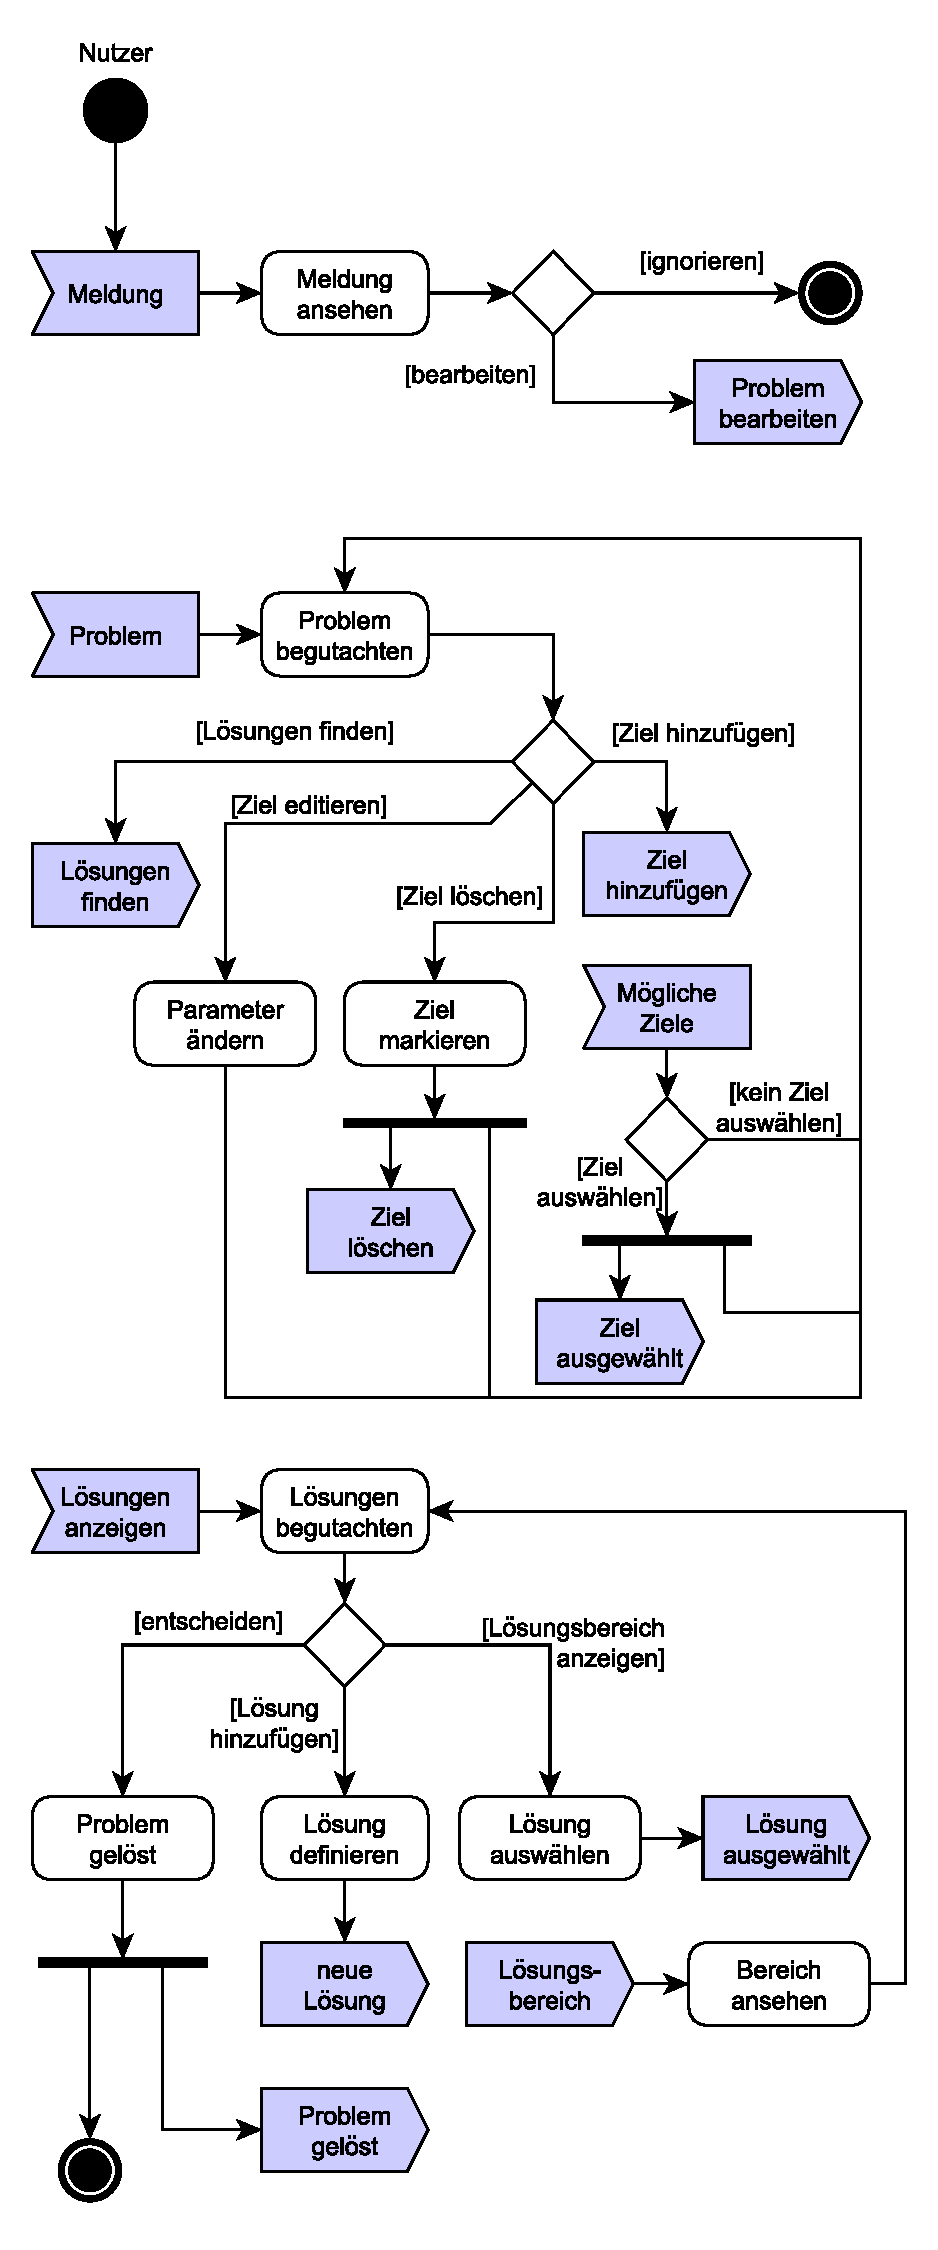
\includegraphics[scale=0.5]{Da_files/UML/Konzept/Aktivitaetsdiagramm-Nutzer.pdf}
\label{pic:Kollaboration-Nutzer}
\caption{Aktivitätsdiagramm: Kollaboration Nutzer}
\end{figure}

\subsubsection*{Interaktionsplattform}
Die Interaktionsplattform stellt die Verbindung zwischen Nutzer und Assistenzsystem dar. Die entsprechenden Verknüpfungen und Aktionen der Interationsplattform sind in Abbildung \ref{pic:Kollaboration-Interaktionsplattform} dargestellt.

\begin{figure}[htbp]
\centering
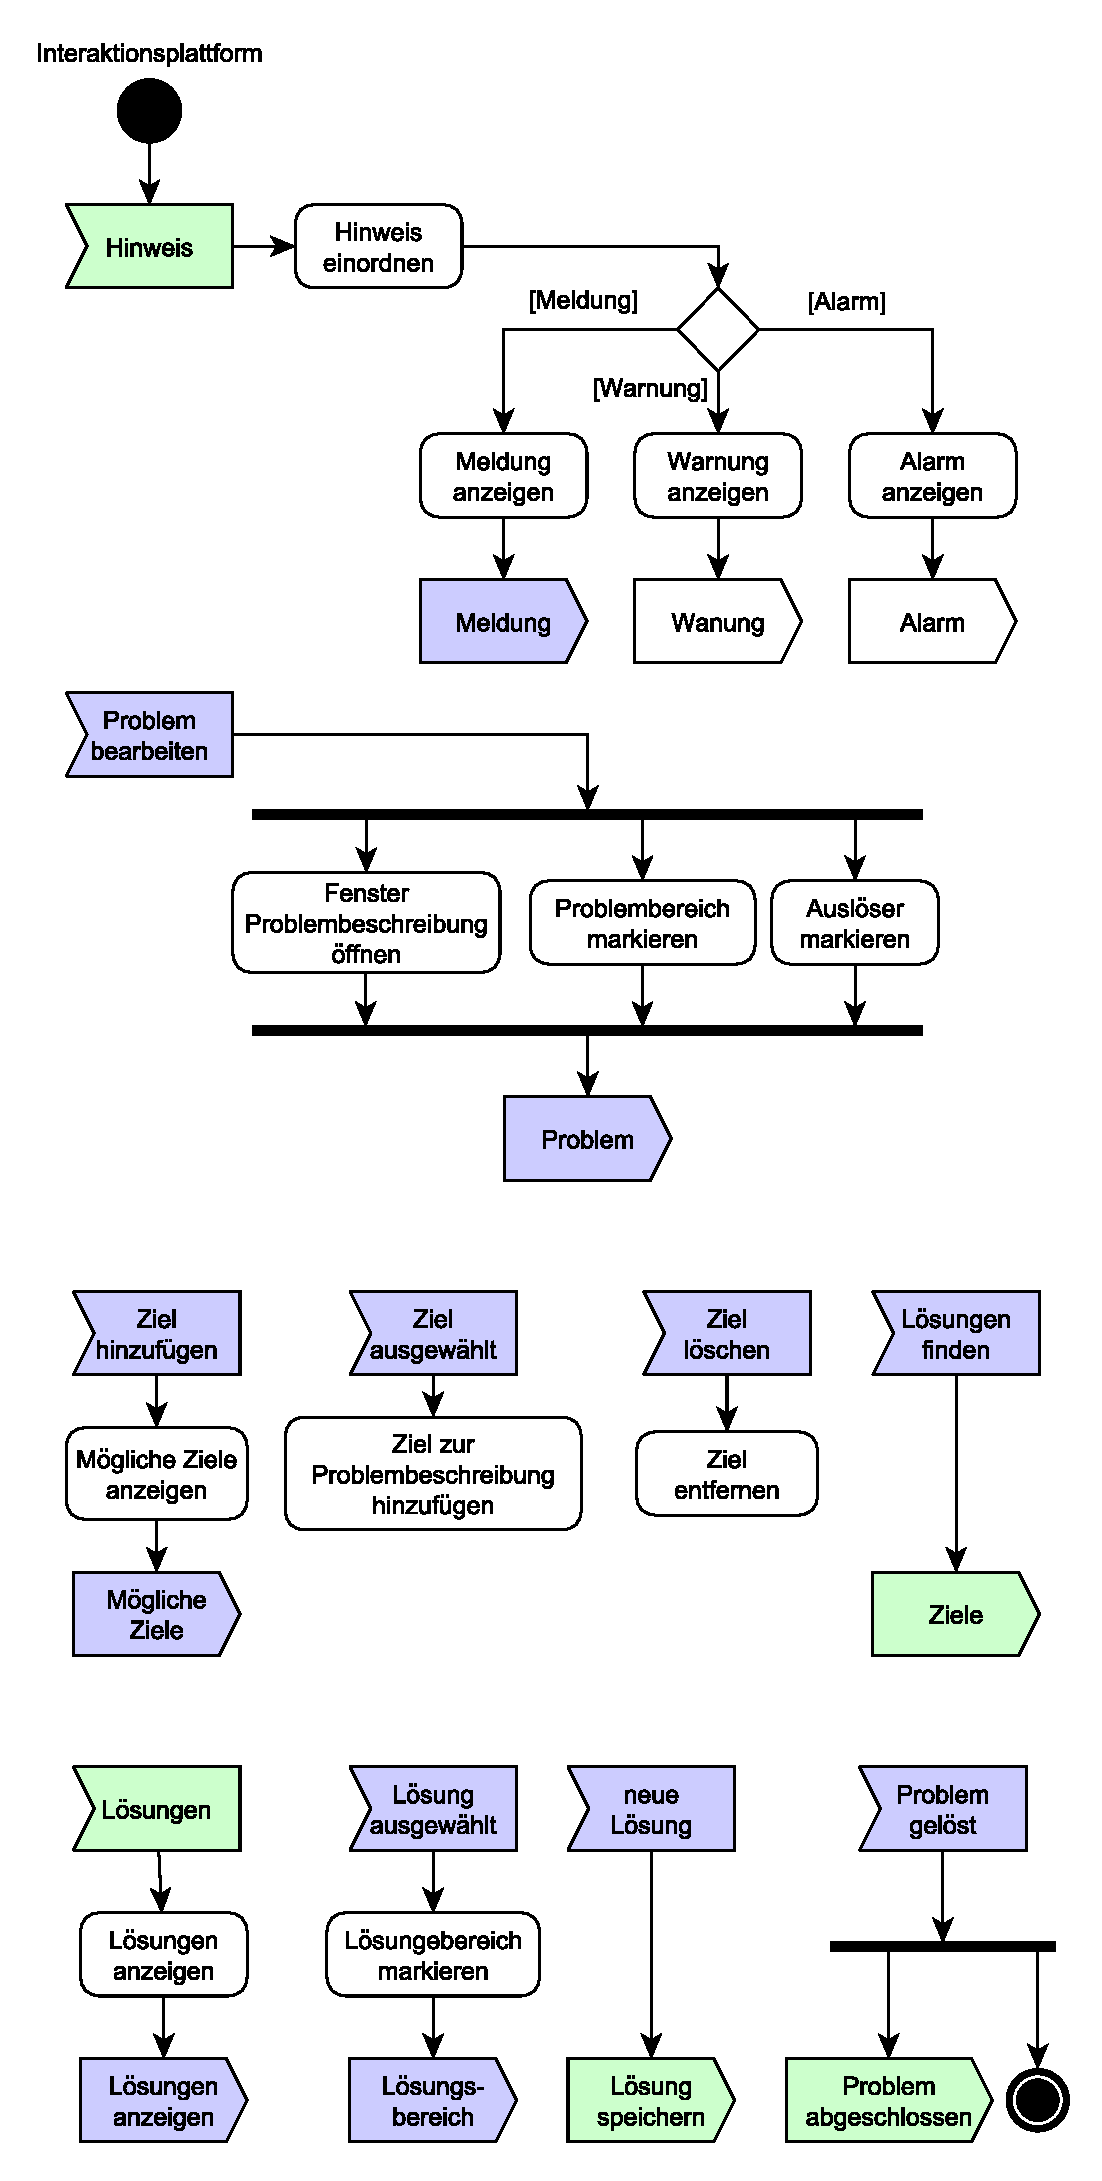
\includegraphics[scale=0.5]{DA_files/UML/Konzept/Aktivitaetsdiagramm-Interaktionsplattform.pdf}
\caption{Aktivitätsdiagramm: Kollaboration Interaktionsplattform}
\label{pic:Kollaboration-Interaktionsplattform}
\end{figure}

\subsubsection*{Assistenzsystem}
Das Assistenzsystem verarbeitet alle zur Verfügung stehenden Informationen und schickt entsprechende Signale an die Interaktionsplattform (siehe Abbildung \ref{pic:Kollaboration-Assistenzsystem}).
\begin{figure}[htbp]
\centering
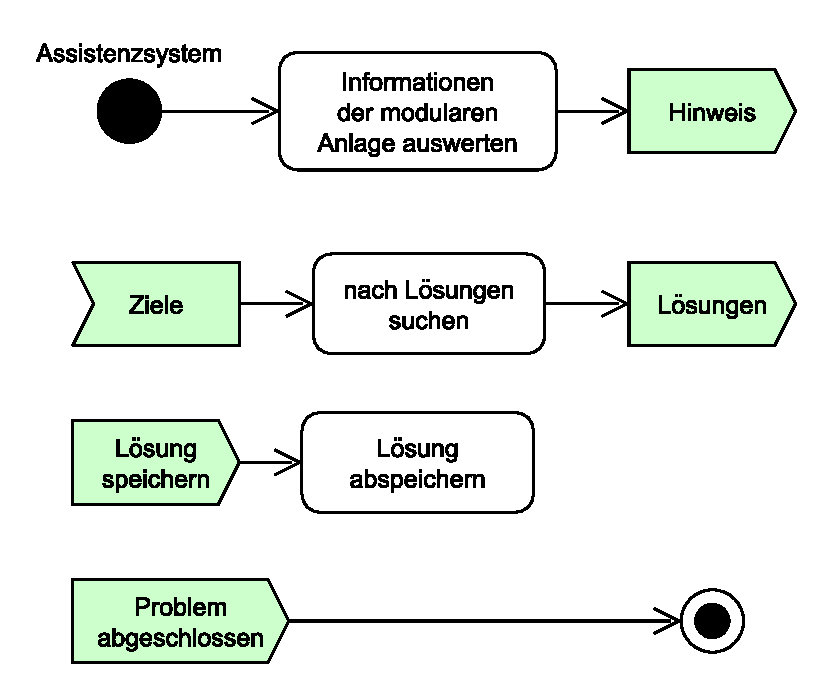
\includegraphics[scale=0.5]{DA_files/UML/Konzept/Aktivitaetsdiagramm-Assistenz.pdf}
\caption{Aktivitätsdiagramm: Kollaboration Assistenzsystem}
\label{pic:Kollaboration-Assistenzsystem}
\end{figure}

\section{Physikalisches Design}
\label{4:Physikalische-Design}
Ausgehend vom konzeptuellen Design wird das physikalische Design entworfen. Es beschreibt die konkrete Darstellung der Funktionen und Informationen. 

\subsection{Prozessführungsebene}
In der bereits existierenden Prozessführungsebene ist der aktuelle Status sichtbar. In Bild \ref{pic:pD-PFE} ist die PFE um eine Meldung erweitert. Über den Button \textbf{Problem bearbeiten} gelangt man zur Problembeschreibung.
\begin{figure}[htbp]
\centering
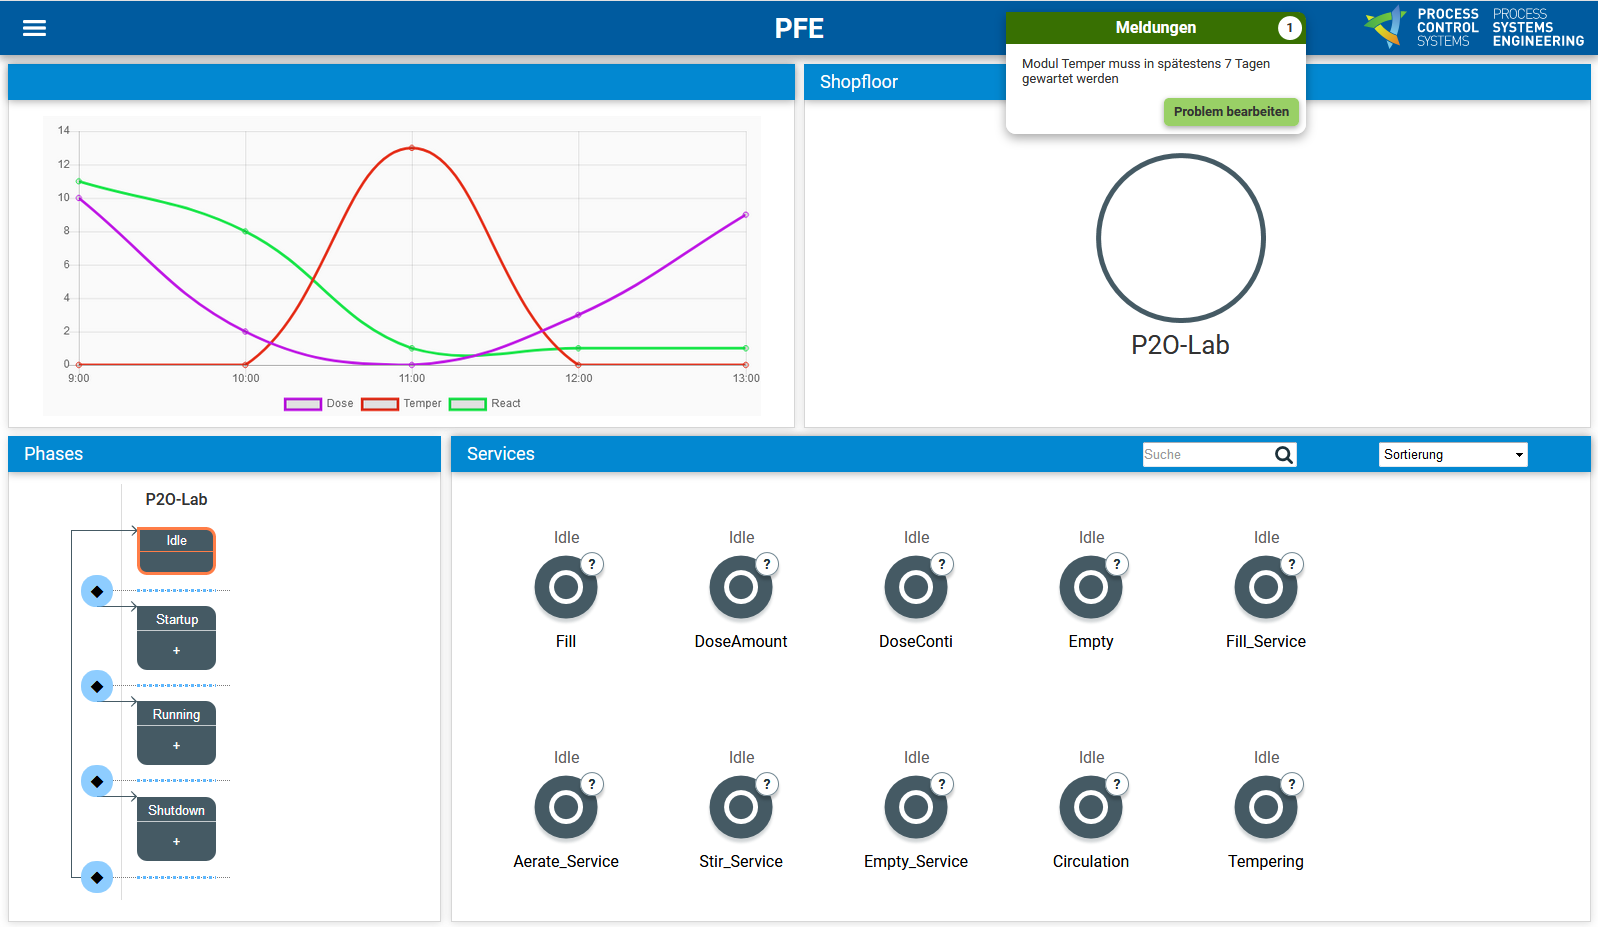
\includegraphics[angle=90, scale=0.47]{DA_files/Bilder/Konzept/Skizze-PFE.png}
\caption{Prozessführungsebene}
\label{pic:pD-PFE}
\end{figure}

\subsection{Problem beschreiben}
Das Feld für die Problembeschreibung ist in zwei Bereiche geteilt (siehe Bild \ref{pic:pD-Problembeschreibung}). Der erste Bereich umfasst die Problembeschreibung und eine (oder mehrere) Spezifikationen. Eine Spezifikation kann z.B. die Dauer der Wartung sein. Diese ist vom Modulherrsteller angegeben und kann nicht verändert werden. Der zweite Bereich stellt die Ziele dar. Über das \textbf{+} ist es möglich Ziele hinzuzufügen (siehe Bild \ref{pic:pD-Problembeschreibung-Ziel-hinzufuegen}). Das Löschen eines Ziels kann durch markieren und anschließendes klicken auf den Mülleimer durchgeführt werden (siehe Bild \ref{pic:pD-Problembeschreibung-Ziel-loeschen}). Neben diesen Fakten wird dem Nutzer auch noch visuell dargestellt, welche Bereiche vom Problem betroffen sind.
Hat der Nutzer alles erfasst und die notwendigen Ziele definiert, so kann er über den Button \textbf{Lösungen finden} das Assistenzsystem nach möglichen Lösungen fragen.

\begin{figure}[htbp]
\centering
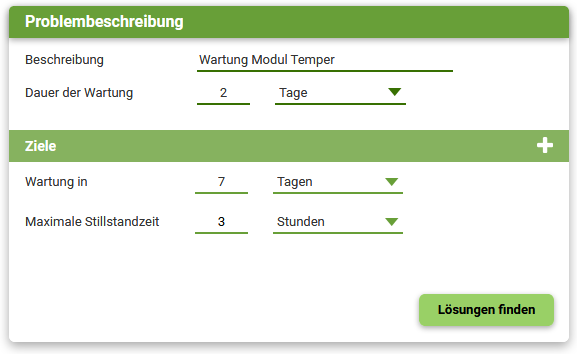
\includegraphics[scale=0.7]{DA_files/Bilder/Konzept/Skizze-Problem-1.png}
\caption{Problembeschreibung}
\label{pic:pD-Problembeschreibung}
\end{figure}

\begin{figure}[htbp]
\centering
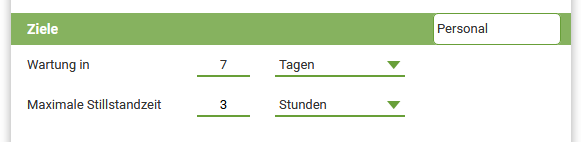
\includegraphics[scale=0.7]{DA_files/Bilder/Konzept/Skizze-Problem-Ziel.png}
\caption{Problembeschreibung - Ziel hinzufügen}
\label{pic:pD-Problembeschreibung-Ziel-hinzufuegen}
\end{figure}

\begin{figure}[htbp]
\centering
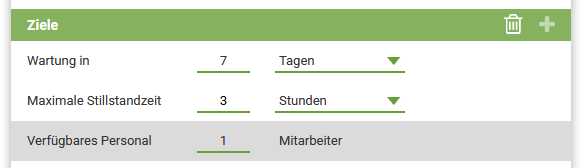
\includegraphics[scale=0.7]{DA_files/Bilder/Konzept/Skizze-Problem-loeschen.png}
\caption{Problembeschreibung - Ziel löschen}
\label{pic:pD-Problembeschreibung-Ziel-loeschen}
\end{figure}

\subsection{Lösungen}
\label{4:pD-Loesungen}
Die eigentliche Frage, in dem gesamten Problemlöseprozess, ist: \glqq Wie kann das Problem gelöst werden?\grqq  \ Dafür stellt das Assistenzsystem mehrere Antworten bereit. Damit der Nutzer diese gut vergleichen kann, sind die verschiedenen Lösungsmöglichkeiten in einer Tabelle dargestellt. In der ganz linken Spalte findet der Nutzer alle Informationen wieder, die bereits in der Problembeschreibung angegeben wurden. Zudem können auch noch weitere Einflussfaktoren, wie Leihkosten und Hinweise durch das Assistenzsystem ergänzt werden, um die Entscheidungsfindung des Nutzers zu erleichtern. Möchte der Nutzer nicht nur Fakten sehen, so werden durch Auswahl einer Lösung auch die Bereiche in der PFE markiert. Beim Ersetzen von einem Modul durch zwei wird sichtbar, welche Bereiche im Rezept angepasst werden müssen (siehe Abbildung \ref{pic:pD-Loesungen}). Hat der Nutzer eine Entscheidung getroffen kann er, nach Auswahl der Lösung, über den Button \textbf{Entscheiden} diese speichern und den Problemlöseprozess beenden.
\begin{figure}[htbp]
\centering
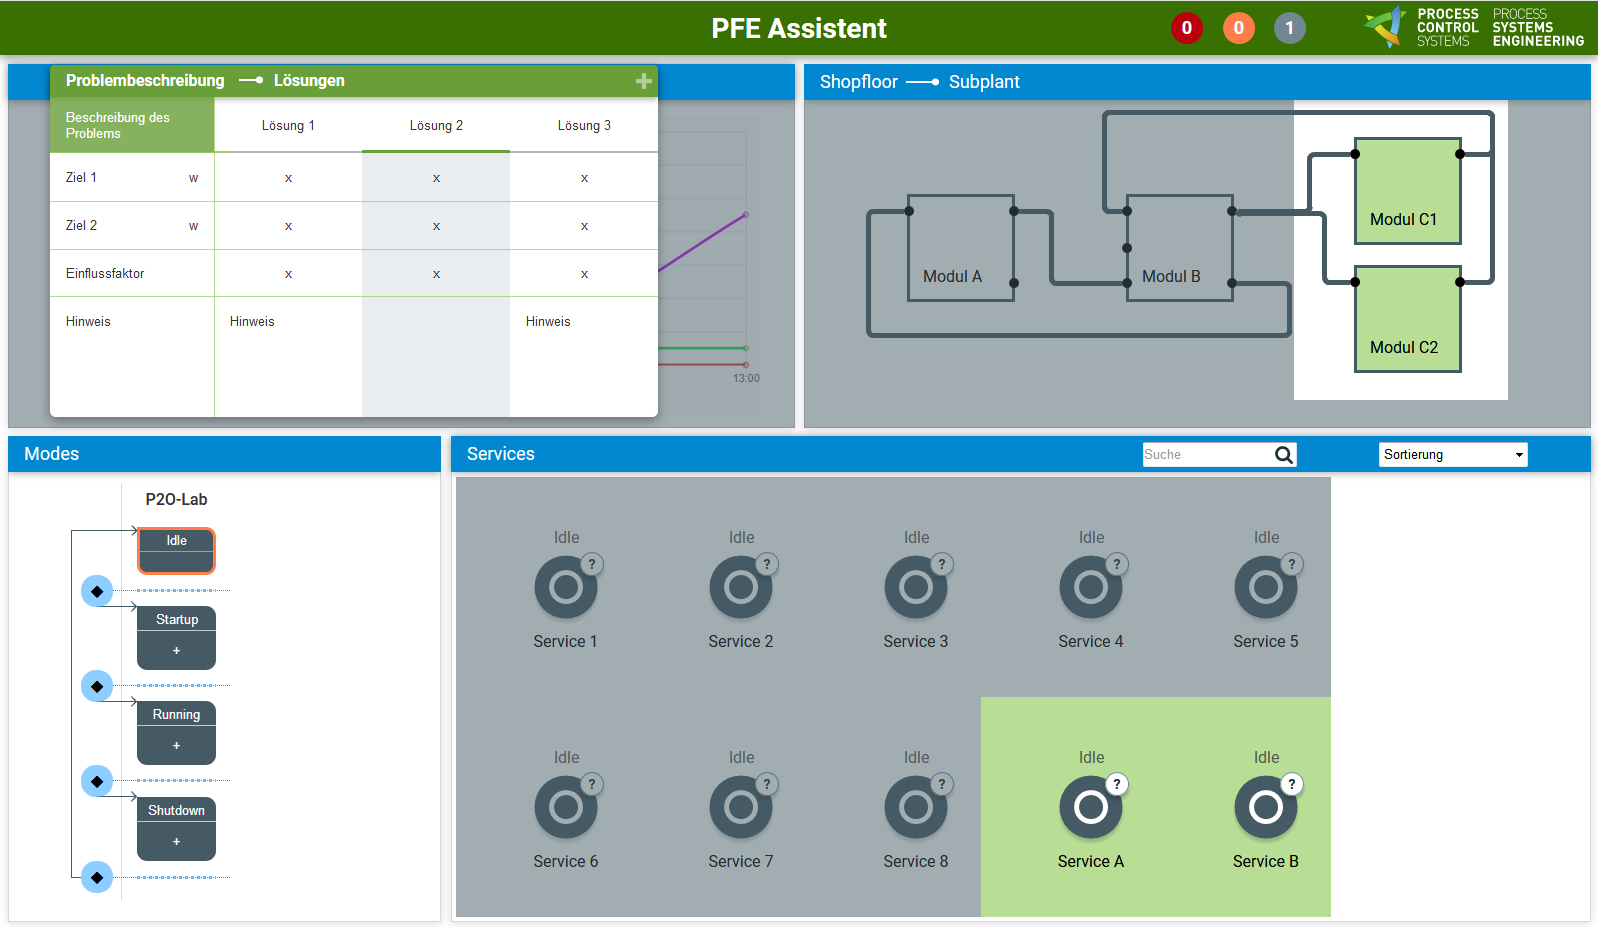
\includegraphics[angle=90,scale=0.47]{DA_files/Bilder/Konzept/Skizze-Loesungen-PFE.png}
\caption{Lösungen für das Problem}
\label{pic:pD-Loesungen}
\end{figure}

\subsection{Entscheidung}
Hat der Nutzer sich für eine Lösung entschieden, so sind keine Änderungen mehr möglich. Die Entscheidung wird hervorgehoben (siehe Bild \ref{pic:pD-Entscheidung} und analog zu den Lösungen auch in der PFE markiert. Das Assistenzsystem könnte aus dieser Entscheidung lernen und so den Wissensschatz erweitern.
\begin{figure}[htbp]
\centering
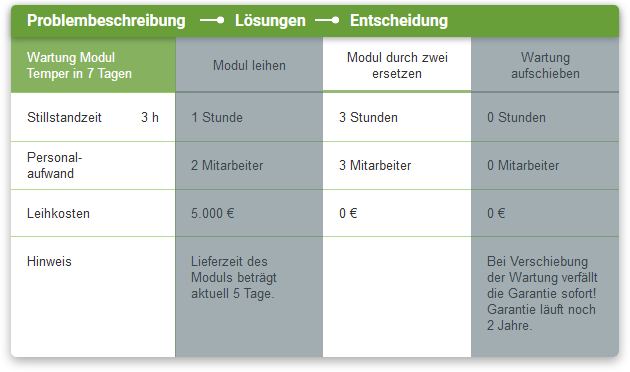
\includegraphics[scale=0.7]{DA_files/Bilder/Konzept/Skizze-Entscheidung.png}
\caption{Entscheidung für eine Lösung des Problems}
\label{pic:pD-Entscheidung}
\end{figure}